\documentclass[12pt]{article}
\usepackage[a4paper, hmargin={2.5cm, 2.5cm}, vmargin={2.5cm, 2.5cm}]{geometry}

\usepackage[utf8]{inputenc}
\usepackage[english]{babel}
\usepackage{amssymb}
\usepackage{amsfonts}
\usepackage{amsmath}
\usepackage{setspace}
\usepackage{algorithm}
\usepackage[noend]{algpseudocode}

%\usepackage[margin=1in]{geometry}
\usepackage{tikz}
\usetikzlibrary{positioning,shapes, shadows, arrows, automata}
%\usepackage[usenames,dvipsnames]{xcolor}

\usepackage{eso-pic} % \AddToShipoutPicture

\usepackage{graphicx}
\usepackage[hidelinks]{hyperref}
\usepackage{float}
\usepackage[danish]{varioref}
\usepackage{multirow}
\usepackage{hhline}
\usepackage{inconsolata}
\usepackage{etoolbox}

\usepackage{fancyhdr}
\usepackage{listings}

%%%%%%%%%%%%%%%%%%%%%%%%%
%         Colors        %

\definecolor{dark-blue}{HTML}{000080}
\definecolor{dark-green}{HTML}{008000}
\definecolor{pale-purple}{HTML}{94558D}
\definecolor{dark-purple}{HTML}{0000AA}
\definecolor{regular-purple}{HTML}{660099}
\definecolor{magenta}{HTML}{B200B2}
\definecolor{light-gray}{HTML}{FAFAFA}
\definecolor{theorem-gray}{HTML}{F0F0F0}
\definecolor{dark-gray}{HTML}{2D2D2D}
\definecolor{comment}{HTML}{808080}
\definecolor{digit}{HTML}{0000FF}

%                       %
%%%%%%%%%%%%%%%%%%%%%%%%%

%%%%%%%%%%%%%%%%%%%%%%%%%
%        Theorem        %

\usepackage{amsthm}
\usepackage{thmtools}
\theoremstyle{definition}

\declaretheoremstyle[
spaceabove=6pt, spacebelow=6pt,
headfont=\normalfont\bfseries,
notefont=\mdseries, notebraces={(}{)},
bodyfont=\normalfont,
postheadspace=1em,
shaded={bgcolor=theorem-gray}
]{exstyle}

\declaretheoremstyle[
spaceabove=6pt, spacebelow=6pt,
headfont=\normalfont\bfseries,
notefont=\mdseries, notebraces={(}{)},
bodyfont=\normalfont,
postheadspace=1em,
shaded={bgcolor=theorem-gray}
]{defstyle}

%\declaretheorem[thmbox=M]{definition}
\declaretheorem[style=defstyle]{definition}
%\declaretheorem[thmbox=M]{example}
\declaretheorem[style=exstyle]{example}

%                       %
%%%%%%%%%%%%%%%%%%%%%%%%%

%%%%%%%%%%%%%%%%%%%%%%%%%
%   subsubsubsection    %

\usepackage{titlesec}
\titleclass{\subsubsubsection}{straight}[\subsection]

\newcounter{subsubsubsection}[subsubsection]
\renewcommand\thesubsubsubsection{\thesubsubsection.\arabic{subsubsubsection}}

\titleformat{\subsubsubsection}
  {\normalfont\normalsize\bfseries}{\thesubsubsubsection}{1em}{}
\titlespacing*{\subsubsubsection}
{0pt}{3.25ex plus 1ex minus .2ex}{1.5ex plus .2ex}

\makeatletter
\def\toclevel@subsubsubsection{4}
\def\l@subsubsubsection{\@dottedtocline{4}{7em}{4em}}
\makeatother

\setcounter{secnumdepth}{4}
\setcounter{tocdepth}{4}

%                       %
%%%%%%%%%%%%%%%%%%%%%%%%%

%%%%%%%%%%%%%%%%%%%%%%%%%
%          Tikz         %

\tikzset{
  treenode/.style = {align=center, inner sep=0pt, text centered,
    font=\sffamily},
  arn_n/.style = {treenode, circle, black, font=\sffamily\bfseries, draw=white, fill=white, text width=1.5em}
}

%                       %
%%%%%%%%%%%%%%%%%%%%%%%%%

%%%%%%%%%%%%%%%%%%%%%%%%%
%       Algorithm       %

\usepackage{xspace}
\usepackage{algpseudocode}
\newcommand*\Let[2]{\State #1 $\gets$ #2}
\newcommand*\Returns[1]{\State \Return #1}
\newcommand{\setalglineno}[1]{\setcounter{ALC@line}{\numexpr#1-1}}
\algrenewcommand\algorithmicrequire{\textbf{Input:}}
\algrenewcommand\algorithmicensure{\textbf{Output:}}
\renewcommand{\algorithmicforall}{\textbf{foreach}}
\algnewcommand{\Or}{\textbf{or}\xspace}
\algnewcommand{\Not}{\textbf{not}\xspace}
\algnewcommand{\In}{\textbf{in}\xspace}

%                       %
%%%%%%%%%%%%%%%%%%%%%%%%%

\setlength\parindent{0pt}
\usepackage[parfill]{parskip}

\newcommand*{\FormatDigit}[1]{\textcolor{digit}{#1}}

\lstset{
	language=Ruby,
	prebreak=\raisebox{0ex}[0ex][0ex]{\ensuremath{\color{red}\space\hookleftarrow}},
	basicstyle=\footnotesize\ttfamily,
	%
	literate=%
    	{0}{{\FormatDigit{0}}}{1}%
        {1}{{\FormatDigit{1}}}{1}%
        {2}{{\FormatDigit{2}}}{1}%
        {3}{{\FormatDigit{3}}}{1}%
        {4}{{\FormatDigit{4}}}{1}%
        {5}{{\FormatDigit{5}}}{1}%
        {6}{{\FormatDigit{6}}}{1}%
        {7}{{\FormatDigit{7}}}{1}%
        {8}{{\FormatDigit{8}}}{1}%
        {9}{{\FormatDigit{9}}}{1}%
        {.0}{{\FormatDigit{.0}}}{2}% Following is to ensure that only periods
        {.1}{{\FormatDigit{.1}}}{2}% followed by a digit are changed.
        {.2}{{\FormatDigit{.2}}}{2}%
        {.3}{{\FormatDigit{.3}}}{2}%
        {.4}{{\FormatDigit{.4}}}{2}%
        {.5}{{\FormatDigit{.5}}}{2}%
        {.6}{{\FormatDigit{.6}}}{2}%
        {.7}{{\FormatDigit{.7}}}{2}%
        {.8}{{\FormatDigit{.8}}}{2}%
        {.9}{{\FormatDigit{.9}}}{2}%
        %{,}{{\FormatDigit{,}}{1}% depends if you want the "," in color
        {\ }{{ }}{1}% handle the space
		{æ}{{\ae}}1
        {ø}{{\o}}1
        {å}{{\aa}}1
        {Æ}{{\AE}}1	
        {Ø}{{\O}}1
        {Å}{{\AA}}1
        {~}{{$\scriptstyle{\sim}$}}1, % handle tilde ~
	%
	%emph={@param,@return},
	otherkeywords={},
	keywords=[2]{self},
	keywords=[3]{__init__},
	keywords=[4]{object},
	keywords=[5]{encoding, flags},
	keywords=[6]{map},
	%
	keywordstyle=\bfseries\color{dark-blue},
	keywordstyle={[2]\color{pale-purple}},
	keywordstyle={[3]\color{magenta}},
	keywordstyle={[4]\color{dark-blue}},
	keywordstyle={[5]\color{regular-purple}},
	keywordstyle={[6]\color{dark-purple}},
	keywordstyle={[7]\bfseries\color{black}},
    commentstyle=\itshape\color{comment},
    identifierstyle=\color{black},
	stringstyle=\bfseries\color{dark-green},
	%emphstyle=\bfseries,
	%
	numbers=left, % where to put the line-numbers
	numberstyle=\ttfamily\color{dark-gray},
	numbersep=5pt, % how far the line-numbers are from the code
	stepnumber=1,
	showstringspaces=false,
	backgroundcolor=\color{light-gray},
	tabsize=4,
	captionpos=b, % sets the caption-position to bottom
	breaklines=true % sets automatic line breaking
}

\linespread{1.3}

%% Change `ku-farve` to `nat-farve` to use SCIENCE's old colors or
%% `natbio-farve` to use SCIENCE's new colors and logo.
\def \ColourPDF {include/ku-farve}

%% Change `ku-en` to `nat-en` to use the `Faculty of Science` header
\def \TitlePDF {include/nat-en}  % University of Copenhagen

\title{
  \vspace{4cm}
  \begin{flushleft}
  \Large{\textbf{Regular Expression Matching In Genomic Data}}
  \vspace{1cm}
  \large{Translating PatScan Patterns into Regular Expressions}
  \end{flushleft}
  \normalsize
  Rasmus Haarslev \texttt{nkh877} \\
  Troels Thomsen \texttt{qvw203} \\
  \textit{\small \today}
  \begin{flushleft}
  \vspace{10cm}
  \small
  {Rasmus Fonseca\\
   Niels Bjørn Bugge Grathwohl\\
   Ulrik Rasmussen\\
   Martin Asser Hansen}
  \end{flushleft}
}

\date{
	%
}

\begin{document}

\AddToShipoutPicture*{\put(0,0){\includegraphics*[viewport=0 0 700 600]{\ColourPDF}}}
\AddToShipoutPicture*{\put(0,602){\includegraphics*[viewport=0 600 700 1600]{\ColourPDF}}}
\AddToShipoutPicture*{\put(0,0){\includegraphics*{\TitlePDF}}}

\clearpage
\pagenumbering{gobble}
\thispagestyle{empty}
\maketitle

\newpage

\begin{center}
\textbf{Abstract}
\end{center}

Scan-For-Matches is the state-of-the-art solution for DNA sequence analysis, which are no longer being maintained. We present an algorithm for translating Scan-For-Matches patterns into regular expressions. By translating into regular expressions, we are able to measure the performance of searching through genomic data on more modern and sophisticated string search engines. We generate a set of regular expressions, and perform an analysis on the performance of these. The analysis looks at the complexity of the original scan-for-matches patterns, and the time it takes to find matches. We discover that the our regular expressions run faster than scan-for-matches for sequences, ranges, as well as low-complexity 'combination' patterns. As complexity of the scan-for-matches 'combination' patterns increases, scan-for-matches shows superior performance. 

\newpage

\tableofcontents
\newpage

\pagenumbering{arabic}
\pagestyle{fancy}
\fancyhf{}
\rhead{\today}
\lhead{Troels Thomsen, Rasmus Haarslev}
\chead{Bachelor Thesis}
\cfoot{\thepage}


\section{Introduction}

The National Institute of Health (NIH) is working on the genetic sequence database, called \emph{GenBank}, which is a collection of DNA sequences. GenBank works together with the DNA DataBank of Japan (DDBJ) and the European Molecular Biology Laboratory (EMBL) to cooperatively collect all publicly available DNA sequences. These three organizations exchange data on a daily basis in what is called the International Nucleotide Sequence Database Collaboration. GenBank is publicizing a new release of their database every two months, and as of April 2015, it consists of approximately 190 billion bases and 182 million sequences~\cite{GenBank}. Parsing and analysing this large amount of data poses several challenges. Searching through the files with simple text search is not advanced enough. DNA contains a lot of redundancy and variation over similar concepts, which means that two seemingly different sequences can have very similar functionality or interact with other components in a similar way. This requires the search functionality to be able to allow for a great deal of variance and flexibility in the sequences which are searched for.

Currently, the state-of-the-art method for searching through genomic data is the scan-for-matches program developed by Ross Overbeek, David Joerg and Morgan Price~\cite{scan-for-matches}, which is able to locate complex DNA patterns, such as looking for a random 8 character sequence, repeated 20 characters ahead, and in reverse. These patterns will be referred to as \textit{patscan patterns}, while the program itself will be referred to as \textit{scan-for-matches}.

While scan-for-matches performs very well, has a very compact language, and is user friendly, the way it is implemented, it is very hard to add new features. Development of scan-for-matches is difficult, which is a problem as it for instance has some unfortunate limitations when running many consecutive scans.

Recently, the KMC group have developed a regular expression implementation, which we will refer to as the KMC engine, which so far has shown competitive performance, compared to current industry standard engines~\cite{two-pass-greedy}. We are hoping that optimized regular expressions running on the KMC engine will be able to match or outperform scan-for-matches.
If we could achieve a performance improvement over scan-for-matches, it would greatly benefit the microbiology team. We see this as a chance to make a unique contribution to ongoing and future research projects, while at the same time providing a chance for the KMC group to have their engine tested in a new scenario.

We wish to determine the possibility of converting sequence analysis patterns used for scan-for-matches~\cite{scan-for-matches}, into regular expressions~\cite{crash-course-regex} and test their efficiency against the KMC~\cite{kmc-website} engine and other industry standard regular expression implementations, such as Google's RE2, Python's RE implementation, and Ruby's RE implementation.

\subsection{DNA/RNA}

Deoxyribonucleic acid (DNA) is a molecule that is found in every known living organism, as well as many viruses. DNA encodes the genetic instructions, that the organism uses in the development and functioning of itself. DNA is a nucleic acid, which is one of three major macromolecules that is essential for all known forms of life.

DNA can generally be described as an alphabet of 4 letters, which represent 4 different nucleobases, adenine (A), thymine (T), cytosine (C), and guanine (G) (figure \ref{dnabases}).

\begin{figure}[H]
\label{dnabases}
\begin{center}
	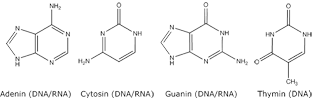
\includegraphics[scale=4]{dnabaserne.png}
\end{center}
\caption{The four different nucleobases found in the DNA nucleotides~\cite{DNA-biotechacademy}.}
\end{figure}

The order of these nucleobases is what decides what function is encoded in any specific strand of DNA. A sequence of these nucleobases (a DNA sequence) is a sort of a genetic blueprint for proteins. During the production of proteins, a DNA sequence is either copied, or transcribed into ribonucleic acid (RNA), which decides which amino acids will be put together, which creates a corresponding protein.

RNA differentiates itself from DNA, among other things, by using uracil (U) instead of thymine. However, uracil and thymine is generally considered synonymous, as both bases binds with adenine.

A DNA strand can bond with another DNA strand containing the complementary nucleobases.

\begin{definition}
\textbf{complementarity} is defined as a nucleobase capable of bonding with another nucleobase.
\begin{center}
\begin{tabular}{|c|c|}
\hline
Base & Complementary base \\
\hline
G & C \\
T/U & A \\
C & G \\
A & T/U \\
\hline
\end{tabular}
\end{center}
\end{definition}

\begin{figure}[H]
	\label{Complementarity}
	\begin{center}
		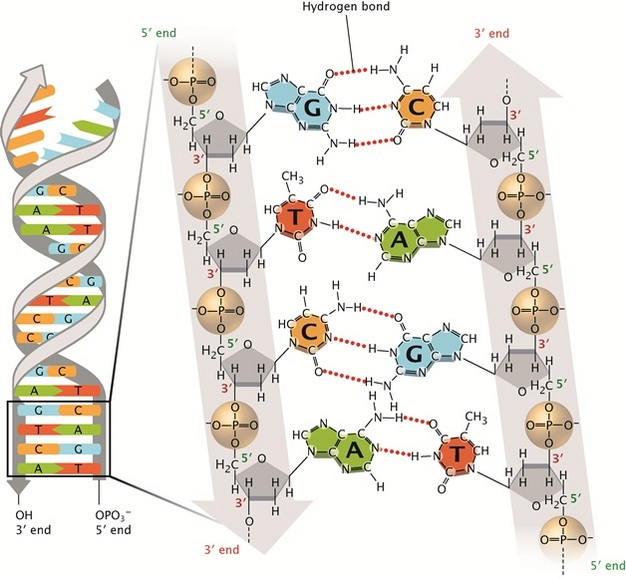
\includegraphics[scale=2.5]{complementarity.jpg}	
	\end{center}
	\caption{This figure shows the hydrogen bonds between the nucleobases, which makes up the basis for complementarity~\cite{DNA-nature}.}
\end{figure}

Sometimes, you may wish to express a DNA sequence's complementary DNA sequence. This is called the complement of a given DNA sequence. The reverse of a complement is called the \textbf{reverse complement}.

\begin{definition}
For a given DNA sequence s, \~{s} is the sequence that contains the complementary bases of s, in reverse order.
\end{definition}

\subsection{Regular Expressions}

In order to talk about regular expressions, we need to be able to talk in general terms of languages. We can define a language as a subset of the infinite set of words or symbols, chosen from a finite alphabet. An alphabet with the letters $\{a,b\}$ might for an example form the words $ab$, $ba$, $aab$ or any such conbination of any length, thus forming an infinite set of words.\\

\begin{definition} An alphabet $\Sigma$ is defined as a finite non-empty set of characters.

\end{definition}

\begin{definition} Given an alphabet $\Sigma$, the language $\mathcal{A}$ is defined by $\mathcal{A} \subseteq \Sigma^*$, where $\Sigma^*$ is the set of all words constructed from alphabet $\Sigma$.
	
\end{definition} 

\begin{definition} Given an alphabet $\Sigma$, we can define a regular expression $E$.\\

	\begin{enumerate}
		\item An expression containing a single letter $a$ from our alphabet $\Sigma$: $E = a$. 
		\item The expression which always matches $E = 1$
		\item The expressions which never matches $E = 0$.
		\item A combination of the two regular expressions $E_1$ and $E_2$:
		\begin{eqnarray}
			E &=& E_1 | E_2 \\
			E &=& E_1E_2 \\
			E &=& E_1^*
		\end{eqnarray}
	\end{enumerate}	
\end{definition} 

\newpage

We can interpret the regular expression $E$ over the alphabet $\Sigma$ as a language denoted by $\mathcal{L}(E)$: \\

\begin{definition} The language $\mathcal{L}(E) \subseteq \Sigma^*$ for the regular expression $E$ from the alphabet $\Sigma$, can be defined as.

	\begin{enumerate}
		\item For single-letter expressions we have
			\begin{eqnarray}
				\mathcal{L}(0) &=& \emptyset \\
				\mathcal{L}(1) &=& \{\epsilon\} \\
				\mathcal{L}(a) &=& \{a\}
			\end{eqnarray}
			Where $a \in \Sigma$
			
		\item For combined expressions we have
			\begin{eqnarray}
				\mathcal{L}(E_1|E_2) &=& \mathcal{L}(E_1) \cup \mathcal{L}(E_2) \\
				\mathcal{L}(E_1E_2) &=& \mathcal{L}(E_1) \odot \mathcal{L}(E_2) \\
				\mathcal{L}(E^*) &=& \bigcup^{\infty}_{n = 0}\mathcal{L}(E^n)
			\end{eqnarray}
			Where $\mathcal{L}(E_1) \odot \mathcal{L}(E_2) = \{w_1w_2 \ |\  w_1 \in \mathcal{L}(E_1), w_2 \in \mathcal{L}(E_2)\}$, and where \\
			$E^0 = 1, \ E^{n+1} = EE^n$.
	\end{enumerate}
\end{definition}


\subsubsection{Implementing regular expressions}

Now that we have defined regular expressions formally, we want to be able to match them against strings. We say that a regular expression $E$ match a string $S$ if $S \in \mathcal{L}(E)$.
The most common way of solving this problem, and also the way industry standard regular expression implementations such as google's RE2 solve this problem~\cite{matching-in-the-wild}, is through expressing the regular expression as a \textit{finite automaton}.\\

\begin{definition} A \textbf{Finite Automaton} can be defined as a five tuple $(Q,\ \Sigma,\ \delta,\ q_0,\ F)$ where
\label{finite automaton defintion}

\begin{itemize}
	\item $Q$ is a finite set of states
	\item $\Sigma$ is an alphabet
	\item $\delta$ is a transition function $\delta \subseteq Q \times (\Sigma \cup \{\epsilon\}) \times Q$
	\item $q_0$ is an initial state $q_0 \in Q$.
	\item $F$ is a set of accepting states $F \subseteq Q$.
\end{itemize}

\end{definition}

For the purpose of representing regular expressions we use two types of finite automata called \textit{deterministic finite automata} or DFA and \textit{non-deterministic finite automata} or NFA. 

\begin{definition} A \textbf{D}eterministic \textbf{F}inite \textbf{A}utomaton can be defined as a Finite Automaton [\ref{finite automaton defintion}] whose transition from a state $q_i$ only has one possible transition candidate state $q_j$
\label{dfa defintion}
\end{definition}
 
An example of definition \ref{dfa defintion} can be seen in figure \ref{dfa_simple}. \\

\begin{figure}[H]
  \begin{center}

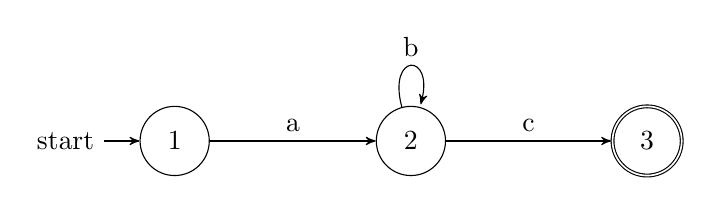
\begin{tikzpicture}[>=stealth', auto, node distance=3cm]
  \node[initial,state] (1) {$1$};
  \node[state] (2) [right of=1] {$2$};
  \node[state,accepting] (3) [right of=2] {$3$};
  
  \path[->] (1) edge node {a} (2);
  %\path[->] (2) edge [bend right] node {c} (3);
  \path[->] (2) edge [loop above] node {b} (3);
  \path[->] (2) edge node {c} (3);
\end{tikzpicture}
	
	\caption{DFA matching the RE \underline{$ab*c$}}
	\label{dfa_simple}
  \end{center}
\end{figure}


\begin{definition} A \textbf{N}on-deterministic \textbf{F}inite \textbf{A}utomaton can be defined as a Finite Automaton [\ref{finite automaton defintion}] whose transition from a state $q_i$ has multiple possible transition candidate states.
\label{nfa defintion}
\end{definition}

An NFA needs to evaluate all possible transition candidates until they reach their final state. If any of the final states is in the set of accepting states $F$, the NFA matches the input string.

\begin{figure}[H]
  \begin{center}

\begin{tikzpicture}[>=stealth', node distance=3cm]
  \node[initial,state] (1) {$1$};
  \node[state] (2) [right of=1] {$2$};
  \node[state] (3) [above of=2] {$3$};
  \node[state] (4) [below of=2] {$4$};
  \node[state,accepting] (5) [right of=2] {$5$};
  
  \tikzset{edge_label/.style={->}} 
  \tikzset{every node/.style={fill=white}} 
  
  \path[->] (1) edge [edge_label] node {a} (2);
  \path[->] (1) edge [edge_label] node {a} (3);
  \path[->] (1) edge [edge_label] node {a} (4);
  \path[->] (2) edge [edge_label] node {b} (5);
  \path[->] (3) edge [edge_label] node {c} (5);
  \path[->] (4) edge [edge_label] node {d} (5);
\end{tikzpicture}
	
	\caption{NFA matching the RE \underline{$ab|c|d$}}
	\label{nfa_simple}
  \end{center}
\end{figure}

In figure \ref{nfa_simple} we see how the NFA can choose between multiple transition candidates upon finding an $a$ in our input sequence, and thus have to try all of them concurrently in order to try to reach our accepting state. \\
It is worth noting that any DFA can be constructed from an NFA but at the cost of exponential blow-up in size~\cite{nfa-to-dfa}.

\newpage

\section{Methods}
\subsection{PatScan as regular expressions}

The most notable of the patscan format's features, is the possibility to search for mismatches, insertions and deletions in a given sequence or stored sequence. The sequence \texttt{AGTCT} can be extended to \texttt{AGTCT[1,1,1]} in order to match up to one mismatch, up to one insertion, up to one deletion or any combination thereof. This means that a sequence of length $n$ with a single mismatch will yield $n^1+1$ possible matches of the data string. \texttt{AGTCT[1,0,0]} will for instance match any of the following, where \_ represents a mismatch.

\texttt{AGTCT, \_GTCT, A\_TCT, AG\_CT, AGT\_T, AGTC\_}

Another powerful feature of patscan is the ability to store a sub-pattern match in a named variable. If a match is found for the named variable in the beginning of a pattern for instance, this match can then be referenced later in the same pattern, by using the variable name. An example of this could be the pattern \texttt{p1=2...4 10...20 {\raise.17ex\hbox{$\scriptstyle\mathtt{\sim}$}}p1}. This pattern will match the contents of \texttt{p1}, followed by any 10 to 20 characters, followed by the match stored in \texttt{p1}, but with the reverse complement as denoted by the \texttt{{\raise.17ex\hbox{$\scriptstyle\mathtt{\sim}$}}}. This is similar to the back-referencing functionality for capturing groups, which many popular regular expression implementations support.%\cite{indsæt citation her.}

Combining this combination notation with the ability to store sequences in variables and matching them further down the pattern, makes the patscan language very compact compared to regular expressions. A pattern as simple as \texttt{p1=8...16 10...50 ~p1[2,0,1]} describes a complex relationship, which cannot easily be discovered through REs.

\subsubsection{Grammar}
\label{Patscan grammar}
Scan-for-patches has an alphabet, which is the set of characters allowed in a patscan sequence. This set is from the nucleobases, that is found in DNA and RNA.
\begin{definition}
The alphabet, that makes up DNA sequences, denoted by $\mathcal{A}_{DNA}$ is:
\begin{center}
$\mathcal{A}_{DNA}$ = \texttt{\{A, T, C, G\}}
\end{center}
\end{definition}

\begin{definition}
The alphabet, that makes up RNA sequences, denoted by $\mathcal{A}_{RNA}$ is:
\begin{center}
$\mathcal{A}_{RNA}$ = \texttt{\{A, U, C, G\}}
\end{center}
\end{definition}

Besides the five basic nucleobases in $\mathcal{A}_{DNA} \cup \mathcal{A}_{RNA}$, 11 ambiguity characters also exist~\cite{DNA-sciencedaily}. These ambiguity characters were designed for positional variations in families of related genes. The ambiguity characters are named so because they represent  an uncertainty of which nucleobases is actually at that spot.

\begin{definition}
The alphabet, that makes up DNA and RNA sequences, as well as the ambiguity characters, denoted by $\mathcal{A}$ is:
\begin{center}
$\mathcal{A}$ = \texttt{\{A, T, U, G, C, Y, R, S, W, K, M, B, D, H, V, N\}}
\end{center}
\end{definition}

The patscan language has the following grammar, and char is any character from the alphabet $\mathcal{A}$.

\begin{figure}[H]
\begin{center}
\begin{tabular}{|lcll|}
	\hline
	$Prog$ & $\rightarrow$ & $StmtSeq$ & \\
	$StmtSeq$ & $\rightarrow$ & list of $Stmt$ & \\
	$Stmt$ & $\rightarrow$ & $Exp$ & \\
	\enspace & $|$ & $LVal1\ =\ Exp$ &  \textcolor{red}{Variable assignment} \\
	\enspace & $|$ & $LVal2$ & \textcolor{red}{Variable usage} \\
	$LVal1$ & $\rightarrow$ & \textbf{Id} & \textcolor{red}{Ids may not be reassigned}\\
	$LVal2$ & $\rightarrow$ & \textbf{Id} $Combi$ & \\
	\enspace & $|$ & {\raise.17ex\hbox{$\scriptstyle\mathtt{\sim}$}} \textbf{Id} $Combi$ & \\
	$Exp$ & $\rightarrow$ & \textbf{num} ... \textbf{num} & \textcolor{red}{Range} \\
	\enspace & $|$ & $Seq\ Combi$ & \\
	$Seq$ & $\rightarrow$ & list of \textbf{char} & \\
	$Combi$ & $\rightarrow$ & [\textbf{num},\textbf{num},\textbf{num}] & \\
	\enspace & $|$ & $\epsilon$ & \\
	\hline
\end{tabular}
\end{center}
\caption{PatScan grammar}
\end{figure}

The patscan language can be broken down into a few simple components or tokens, which we will refer to as sub-patterns. We have divided the sub-patterns into the following classes:

The sub-patterns, that consists only of a consecutive sequence of characters from $\mathcal{A}$, is denoted as a \textbf{sequence} (Example: \texttt{AGTCT})

The sub-patterns, that consists of a consecutive sequence of characters from $\mathcal{A}$, followed by square brackets, containing three numbers (each representing \textbf{mismatches}, \textbf{deletions}, and \textbf{insertions} respectively), is denoted as a \textbf{combination sequence} (Example: \texttt{AGTCT[1,0,0]})

The sub-patterns, that consists of a number, $a \geq 0$, followed by exactly three dots, followed by a number, $b \geq a$, is denoted as a \textbf{range} (Example: \texttt{2...4})

The sub-patterns, that consists of a string, denoted as a \textbf{variable name}, followed by an equal sign, and then a \textbf{sequence}, is denoted as a \textbf{variable assignment} (Example: \texttt{p1=AGTCT})

The sub-patterns, that consists only of a \textbf{variable name}, is denoted as a \textbf{variable usage} (Example: \texttt{p1})

The reverse complement of a sequence or variable is denoted by placing a \texttt{{\raise.17ex\hbox{$\scriptstyle\mathtt{\sim}$}}q1} directly in front of the sequence or variable.


\subsubsection{Ranges}

Patscan ranges are very similar to RE ranges, and is therefore easily translated. A patscan range, which has the following form:
\begin{equation}
\label{example:range}
	2...5
\end{equation}
It translates into 'from 2 to 5 of any character'. In the general syntax of RE, there is a character for 'any character', which is \texttt{.}, and a quantifier, where you can state how many of a given character you want matched, which is \texttt{\{min,max\}}. Using these, (\ref{example:range}) translates into the following RE:
\begin{equation}
.\{2,5\}
\end{equation}

\subsubsection{Mismatches, Deletions, and Insertions}

Combination sequences do not exist in REs. One way to represent these sub-patterns as REs is by constructing every possible combination of the sequence, matching the patscan notation, which is the problem we sought to solve.

A recursive algorithm $f$ that solves this problem can easily be written, but it will have a running time of exponential growth, when the length of the sequence increases. The way this is done, is by looking at each letter in the sequence, and branch out for each choice of mismatch, deletion or insertions for the given letter.

\begin{example}[label=example:recursion]
Looking at the combination sequence \texttt{AGCTC[2,0,0]}, we start by taking the \texttt{A}, and call $f$ with the remaining letters for every possibility of the \texttt{A}.
\begin{eqnarray}
	Left\ branch &=& f(\texttt{A}, \texttt{GCTC[2,0,0]}) \\
	right\ branch &=& f(mismatch(\texttt{A}), \texttt{GCTC[1,0,0]})
\end{eqnarray}
The left branch will continue recursively with \texttt{GCTC[2,0,0]}, and the right branch will do the same but with only one mismatch available, since we already chose \texttt{A} as our first mismatch. When $f$ reaches base case, we will have a string with a unique combination of mismatches. Like this, all possible combinations will be constructed, and they can be added to a list of all combinations.
\end{example}

Adding deletions and insertions to \textbf{example \ref{example:recursion}} will increase the number of possibilities for each letter, thus increasing the amount of recursion. The recursion does not stop until every combination is found, which means that if the sequence is large enough (This can happen already at a length of 20, if not earlier, depending on the number of mismatches, insertions, and deletions), the program can reach maximum recursion depth (depending on the programming language), or run out of memory before terminating.

In order to guarantee a low recursion depth, we use a divide and conquer algorithm~\cite{Algorithms} instead, that reduces the recursion depth to $log(n)$. This works by splitting the sequence in two halves per recursion, such that at the deepest recursion level, we have sequences of only a single character, as can be seen in figure \ref{fig:tree_example}. 

\begin{figure}[H]
\begin{tikzpicture}[->,>=stealth',level/.style={sibling distance = 5cm/#1,
  level distance = 1.5cm}] 
\node [arn_n] {abcd}
	child{ node [arn_n] {ab} 
		child{ node [arn_n] {a}}
		child{ node [arn_n] {b}}                            
	}
    child{ node [arn_n] {cd}
		child{ node [arn_n] {c}}
		child{ node [arn_n] {d}}
	}
; 
\end{tikzpicture}
	\centering
	\caption{Tree structure, showing the steps taken by the algorithm during the divide step.}
	\label{fig:tree_example}
\end{figure}

After dividing the sequence into characters, and we reach \emph{base case}, we have to 'conquer' each sub-problem. On the lowest recursion level (where the sequence is a single character), algorithm~\ref{alg:divideandconquer} will make a list of all possibilities, which that character can be.

\begin{example}[label=example:possibilities]
When reaching base case for a character $a$, algorithm~\ref{alg:divideandconquer} will construct the following possibilities for mismatches and deletions

\begin{center}
	\texttt{a, \^{}a, \_}
\end{center}

\noindent as well as the following for insertions

\begin{center}
	\texttt{.\{1\}a, .\{2\}a, $\cdots$, .\{n\}a} \\
	\texttt{a.\{1\}, a.\{2\}, $\cdots$, a.\{n\}}
\end{center}

\noindent This list of possibilities for $a$ represents that $a$ may take the form of a mismatch (\texttt{\^{}a}), its original form, or any of the other forms in the lest, This list of possibilities is then returned, and it can be combined with the list received from the 'b' recursion.
\end{example}

\emph{Combining} two such lists means that each element in the left list is concatenated behind each element in the right list. Like so, a new list of size $m x n$ will be created. The total number of mismatches, deletions, and insertions are being kept track of, and if combining two elements will result in more mismatches, deletions, or insertions than the maximum allowed, it is skipped.

\begin{spacing}{0.8}
\begin{algorithm}[H]
	\caption{find\_combinations}
	\label{alg:divideandconquer}
  	\begin{algorithmic}[1]
    		\Require
    			\Statex $seq$ - sequence string to be translated
    			\Statex $m_{max}$ - allowed number of mismatches
    			\Statex $d_{max}$ - allowed number of deletions
    			\Statex $i_{max}$ - allowed number of insertions
    		\Ensure
    			\Statex List of all possible combinations
		\Statex
		\Function{find\_combinations}{$seq$, $m_{max}$, $d_{max}$, $i_{max}$}
    		\If{$seq.length > 1$}
    			\Let{left\_tree}{\Call{find\_combinations}{seq[0..(seq.length/2).floor-1], $m_{max}$, $i_{max}$, $d_{max}$}} \label{alg:divide:leftT}
    			\Let{right\_tree}{\Call{find\_combinations}{seq[(seq.length/2).floor..-1], $m_{max}$, $i_{max}$, $d_{max}$}} \label{alg:divide:rightT}
    		\Else
    			\Returns{List of all mismatch, insertion, and deletion combinations of seq} \label{alg:divide:conquer}
    		\EndIf
    		\State
    		\Let{combined}{empty list}
    		\Let{unique\_combinations}{empty set}
    		\ForAll{LL \In left\_tree} \Comment{LL: Left leaf}
    			\ForAll{RL \textbf{in} right\_tree} \label{alg:divide:inner} \Comment{RL: Right leaf}
    				\If{$LL.m + RL.m > m_{max}$ \Or $LL.d + RL.d > d_{max}$ \Or $LL.i + RL.i > i_{max}$} \label{alg:divide:invariant1}
    					\State continue
    				\EndIf
    				\If{\Not LL.seq + RL.seq \In unique\_combinations.keys} \label{alg:divide:invariant2}
    					\Let{unique\_combinations}{LL.seq + RL.seq}
    					\Let{combined}{LL + RL}
    				\EndIf
    			\EndFor
    		\EndFor
    		\Returns{combined}
    		\EndFunction
  	\end{algorithmic}
\end{algorithm}
\end{spacing}


\subsubsubsection{Correctness}

We wish to show that algorithm~\ref{alg:divideandconquer} is correct, by showing that given a set of parameters, that meets a pre-condition, algorithm~\ref{alg:divideandconquer} will arrive at a result, that satisfies a post-condition. Additionally, we must also make sure, that algorithm~\ref{alg:divideandconquer} satisfies an invariant in all iterations.

Pre-conditions:
\begin{itemize}
\item[-] seq is a string of length $i > 0$
\item[-] $m_{max}$ is a non-negative integer
\item[-] $d_{max}$ is a non-negative integer
\item[-] $i_{max}$ is a non-negative integer
\end{itemize}

post-condition:
\begin{itemize}
\item[-] The list $combined$ contains all combinations of the initial sequence with up to  $m_{max}$ mismatches, $d_{max}$ deletions, and $i_{max}$ insertions.
\end{itemize}


We start by showing the correctness of the inner loop. For this, we have the following loop invariant, which must be satisfied during all iterations of the loop.

\textbf{For an element $a$, and another element $B[j]$, a combination of the two yields a new unique element $c$, such that it satisfies $c_m \leq m_{max}$, $c_d \leq d_{max}$, $c_i \leq i_{max}$, where $c_m$, $c_d$, $c_i$ is the number of $c$'s mismatches, deletions and insertions respectively.}

\begin{itemize}
\item Initialization:
\begin{itemize}
	\item[] Prior to the loop at line~\ref{alg:divide:inner}, the invariant is respected (trivially), as $B[j]$ is \textbf{null}.
\end{itemize}

\item Maintenance:
\begin{itemize}
	\item[] For $j = k$, the loop will have an element $a$ (\texttt{LL} in the algorithm), and an element $B[j]$ (RL in the algorithm), which both respect the condition in the invariant. Before combining $a$ and $B[j]$, the condition in the invariant is checked at line~\ref{alg:divide:invariant1} and line~\ref{alg:divide:invariant2}, and if it is not satisfied, the combining of $a$ and $B[j]$ is skipped.
\end{itemize}

\item Termination:
\begin{itemize}
	\item[] When the loop terminates, the invariant will be true on the output.
\end{itemize}
\end{itemize}

Since the invariant is satisfied for the inner loop, meaning it is correct, the same can be concluded for the outer loop, as it iterates over iterations of the inner loop, which means the invariant for the outer loop can be seen as multiple of the inner loop's invariant.


Next, we want to show that the recursion is correct. For this we have the invariant $I(n)$:

\textbf{For a set $A$, and a set $B$, a combination of the two, where each element in $A$ is combined with each element in $B$ separately, yields a set $C$, such that all $e \in C$ satisfies $e_m \leq m_{max}$, $e_d \leq d_{max}$, $e_i \leq i_{max}$, where $e_m$, $e_d$, $e_i$ is the number of $e$'s mismatches, deletions and insertions respectively.}


\begin{itemize}
\item Initialization:
\begin{itemize}
	\item[] Prior to the recursion step at line~\ref{alg:divide:leftT} and line~\ref{alg:divide:rightT}, the invariant is respected (trivially), as set $A$ and $B$ are empty..
\end{itemize}

\item Maintenance:
\begin{itemize}
	\item[] For combining at step $k$, the algorithm will have two sets of valid elements (respects the condition in the invariant), from which it will construct a new set of all combinations of the elements in the two original sets. This combining follows the invariant of the inner loop, and will thus also respect the recursion invariant.
\end{itemize}

\item Termination:
\begin{itemize}
	\item[] When the recursion terminates, the invariant will be true on the entire output.
\end{itemize}
\end{itemize}


\subsubsubsection{Redundancy}

Using algorithm \ref{alg:divideandconquer} without modifications, we will have a lot of redundancy when translating insertions. This comes from the fact, that we wish to construct all possible combinations, and that we do it recursively.

If we look at the combination sequence \texttt{ab[0,0,1]}, the possible outcomes of \texttt{a} (at the lowest level of recursion) can be \texttt{a}, \texttt{.a}, and \texttt{a.}, and the same for \texttt{b}. Combining these, we will have two different cases of \texttt{a.b} (\texttt{a. b} and \texttt{a .b}). It is redundant to keep both, and by keeping it, will create exponentially more redundancy, the more levels of the recursion there is.

Assuming we have an even number of characters in the sequence, and that only insertions are allowed, we have that on the first 'combine' step, there is
\begin{eqnarray}
	\label{r_0}
	r_0 = \frac{1}{2}n\sum^{i_{max}}_{i=1} i
\end{eqnarray}

redundant cases, where $\frac{1}{2}n$ is the number of combine steps in this recursion level.

\begin{example}
The following example shows the variations of a with b that are the same when combined. The bold characters are combined with the cursive characters.
\begin{eqnarray}
	i_{1}: \textbf{a.}b\ \ \textbf{a}.b = 2 - 1 = 1 \\
	i_{2}: \textbf{a..}b\ \ \textbf{a.}.b\ \ \textbf{a}..b = 3 - 1 = 2 \\
	i_{3}: \textbf{a...}b\ \ \textbf{a..}.b\ \ \textbf{a.}..b\ \ \textbf{a}...b = 4 - 1 = 3
\end{eqnarray}
Here, for $i_{1}$, we have 2 cases, that are the same. One of those are redundant, thus $2 - 1 = 1$ redundant case. \\
Since all cases for $i_{n-1}$ also applies to $i_{n}$, we end up with
\begin{eqnarray}
	\sum_{i=1}^{i_{max}}i
\end{eqnarray}
redundant cases for each combination step in each branch, where $i_{max}$ is the maximum number of insertions. If $n$ is the number of characters in the sequence, there are $\frac{1}{2}n$ combination steps on this level, which gives us:
\begin{eqnarray}
	r_0 = \frac{1}{2}n\sum^{i_{max}}_{i=1} i
\end{eqnarray}
\end{example}

On the next combine step, we have $r_1$ redundant cases. In order to calculate $r_1$, I will define $c = 1 + 2i$ as the number of cases in the \textit{base case}, meaning the number of cases in the lowest level of recursion. Each redundant case will be combined with all cases in the second set, which contains $c^2$ cases. All non-redundant cases from the first set will also be combined with all redundant cases of the second set. 

Because there is maximum of the number of insertions allowed in a single case, where this maximum varies, a lot of combinations will be skipped, resulting in fewer cases than $c^2$. To correct for this, we will introduce a factor $\kappa$, that represents the scaling factor, that corrects the number of elements in a given set, corresponding to the number of insertions allowed.
\begin{eqnarray}
	\label{r_1}
	r_1 = \frac{1}{4}n(2r_0\frac{c^2}{\kappa_1} - r_0^2)
\end{eqnarray}

\begin{example}
We have a set $A$ and another set $B$, each containing $\frac{c^2}{\kappa}$ elements, of which $r_0$ are redundant.

All $r_0$ redundant elements in $A$ will combine with all elements in $B$, creating $r_0\frac{c^2}{\kappa}$ redundant cases. Likewise, all $\frac{c^2}{\kappa}-r_0$ non-redundant case in $A$ will combine with all $r_0$ redundant cases in $B$, creating $r_0(\frac{c^2}{\kappa}-r_0)$ additional redundant cases. There are $\frac{1}{4}n$ combination steps on this level, which gives us:
\begin{eqnarray}
	r_1 &=& \frac{1}{4}n(r_0\frac{c^2}{\kappa_1} + r_0(\frac{c^2}{\kappa_1} - r_0))\\
		&=& \frac{1}{4}n(r_0\frac{c^2}{\kappa_1} + r_0\frac{c^2}{\kappa_1} - r_0^2))\\
		&=& \frac{1}{4}n(2r_0\frac{c^2}{\kappa_1} - r_0^2)
\end{eqnarray}
\end{example}

We can then calculate the total amount of redundancy of any sequence with $logn$ recursion depth, via induction:
\begin{eqnarray}
	r_x &=& \frac{1}{2^{x+1}}n (r_{x-1}\frac{c^{2^{x+1}}}{\kappa_x} + r_{x-1}(\frac{c^{2^{x+1}}}{\kappa_x} - r_{x-1}))\\
		&=& \frac{1}{2^{x+1}}n (r_{x-1}\frac{c^{2^{x+1}}}{\kappa_x} + r_{x-1}\frac{c^{2^{x+1}}}{\kappa_x} - r_{x-1}^2)\\
		\label{r_x}
		&=& \frac{1}{2^{x+1}}n (2r_{x-1}\frac{c^{2^{x+1}}}{\kappa_x} - r_{x-1}^{2^{x+1}})
\end{eqnarray}

Here, $x$ is the recursion depth, and will thus go up to $logn$, where $n$ is the length of the patscan sequence.

Given a pattern, where mismatches and deletions are allowed as well as insertions, the amount of redundancy increases, as $c$ will become larger.

Despite result reached in formula \ref{r_x}, inaccuracy occurs, as the recursion depth varies in the recursion branches based on the length of the original string, like in figure \ref{fig:recursion_depth_example}.

\begin{figure}[H]
\begin{tikzpicture}[->,>=stealth',level/.style={sibling distance = 5cm/#1,
  level distance = 1.5cm}] 
\node [arn_n] {abc}
	child{ node [arn_n] {a}}
    child{ node [arn_n] {bc}
		child{ node [arn_n] {b}}
		child{ node [arn_n] {c}}
	}
; 
\end{tikzpicture}
	\centering
	\caption{Tree structure showing how recursion depth varies in different branches.}
	\label{fig:recursion_depth_example}
\end{figure}

Despite of this inaccuracy, it is still trivial, that the amount of redundancy in is excessive, as it translates directly into additional running time.

Avoiding this redundancy is very important, and relatively trivial. Every time two cases are combined, it is put in a set, and we can thus avoid having duplicates. By avoiding duplicates in early on in algorithm~\ref{alg:divideandconquer}, we will have far fewer operations later, which saves us a lot of memory and running time.


\subsubsection{Variable assignments \& usage}

Variable assignment is when you have a pattern of some sort, that you assign to a variable, so that it may be reused later. Any kind of non-variable pattern may be used in a variable pattern. Hence, we have three different variable assignments:

\texttt{p1=ATCG} \\
\texttt{p2=ATCG[2,0,0]} \\
\texttt{p3=2...4}

These assignments can be referenced by using the variable name. An example of such usage could be

\texttt{q1=ACCT 2...5 q1}

In addition to referencing the variable, a variable may also be inverted. This is denoted by using a tilde character prepended to the variable:

\texttt{{\raise.17ex\hbox{$\scriptstyle\mathtt{\sim}$}}q1}

Here, inversion refers to the reverse complement of the sequence stored in the variable.

Sequence and combination assignments are implemented by translating the sequence/combination and storing the translated regular expression in a table, with the variable name as the key. Then, if the variable is used later in the patscan pattern, the translated sequence/combination may be placed into the full regular expression. This way, there are no actual referencing in the regular expression, keeping the expressions regular.

Assignment of a range is something we have chosen not to implement, as it can't be implemented without the use of back-referencing. This is because there's no way of knowing what a range will actually be besides x-y random characters. Because of this inherent ability to change, depending on where in the file the engine is matching, it is not possible to 'hard code' it as a regular expression.

Using back-referencing in our implementation will cause our RE patterns to lose regularity, and with that, performance.


\subsection{Running time}

In the divide step, our algorithm (algorithm \ref{alg:divideandconquer}) first splits a given sequence in half multiple times until it reaches base case (where length of the sequence is one). It does this recursively with a branching factor of two, meaning the running time so far is 
\begin{eqnarray}
	T(n) = 2T(\frac{n}{2}) = O(log_2n)
\end{eqnarray}

The conquer step, where we construct each combination of every base case, is trivially solved by constructing a set of the combinations. It constructs one element if any mismatches are allowed, which it can do in $O(1)$ constant time. It constructs one element if any deletions are allowed, which it can also do in $O(1)$ constant time. It constructs two elements for each insertions that is allowed, which take $O(2i)$ time, where $i$ is the number of insertions allowed. It does this for every base case, which leaves us with a total running time of $O(ni)$.
\begin{eqnarray}
	T(n) = O(log_2n) + O(ni)
\end{eqnarray}

In the combine step, we combine each element of two sets $A$ and $B$. Each combination takes $O(1)$ constant time, and it does this operation $|A| \cdot |B|$ times. The sets $A$ and $B$ were created in the same way recursively, which means the total running time of each recursion level increases exponentially. In total we have a running time of $O(i^n)$, where $i$ is the number of insertions, and $n$ is the length of the sequence.

The running time of every combination step before the final one combined is significantly smaller than the final combination step, which means that they are consumed by the exponentially larger running time of the last iteration. This gives us a running time of:
\begin{eqnarray}
	T(n) = O(log_2n) + O(ni) + O(i^n)
\end{eqnarray}

The running time of the divide and conquer step also consumed by the combine step, leaving us with a running time of
\begin{eqnarray}
	O(i^n)
\end{eqnarray}

\newpage

\subsection{Data Analysis}

We have chosen chromosome number 22 from the human genome. Chromosome 22 is the smallest chromosome in the human genome making it better suited for testing. Our version of chromosome 22 contains a lot of noise in the form of N's, specifying unknown bases during sequencing.~\cite{human-genome} We have decided not to modify the contents of the fasta file, since we want our tests to be close to a realistic use scenario.

We could possibly have removed the N's and the linebreaks from the fasta file, in order to reduce the file size and thus reduce the runningtime of the regular expressions which we generate. However we felt that this would not significantly improve our results, and also make our test further from a real-world scenario.

\section{Results}

\subsection{Experiment design}

We have set up a testing environment for our regular expressions, which consists of a series of patscan patterns. These patterns are grouped as mismatches, insertions, deletions, mixed combinations and ranges. Each group contains roughly 10 pattern files with increasing complexity such that we test both simple and advanced patterns which in term become larger regular expressions. Here, complexity refers to the complexity of the patscan patterns, which we have defined as the length of the sequence. In case of multiple patterns with the same sequence length, their respective allowed number of deletions, insertions, deletions will act as tie breaker. Patscan pattern complexity are thus not to be associated with RE complexity (which we define as the length of the RE), as a patscan pattern with some complexity, may be translated into a RE with a lower RE complexity (length) than another RE, which was translated from a patscan pattern with lower patscan pattern complexity than the former. We run each group against our chosen regular expression implementations which include Ruby, Python, google's RE2~\cite{re2} and KMC.
 
Each pattern file is translated using our ruby implementation of the algorithm described in algorithm~\ref{alg:divideandconquer}. The resulting regular expressions is subsequently stored in a file and passed as an argument to the regular expression implementation. In most cases we have made a small wrapper program which takes a .re file and a .fa file, and actually performs the matching using the given implementation. Each patscan file is parsed in its own thread in order to take advantage of our multicore / multithreaded testing computers. Each thread is also given a time limit of 15 minutes after which the thread is killed. This time limit is given for two reasons. First of all we suspect that some of the regular expressions might never (or close to never) finish, and second of all the difference between taking 15 minutes and 20 minutes is insignificant compared to scan-for-matches' in-the-seconds running time, and thus the program might as well never finish.

The outputs of our wrapper programs are piped to a result file for each regular expression implementation and subsequently each pattern. 

\subsection{Experiment results (TO BE WRITTEN)}

In the following, we will make an analysis of how well our translated REs perform on various RE implementations compared to the performance of scan-for-matches. In the analysis, we will show various plots of our performance results. For some of our tests, the REs become large enough, that limits in some of the RE implementations stops them from compiling the REs. When this happens, our test returns a match time of 0. This means that in some of our graphs, 

\subsubsection{Mismatches}

We notice that even for 

\begin{figure}[H]
	\label{Complementarity}
	\begin{center}
		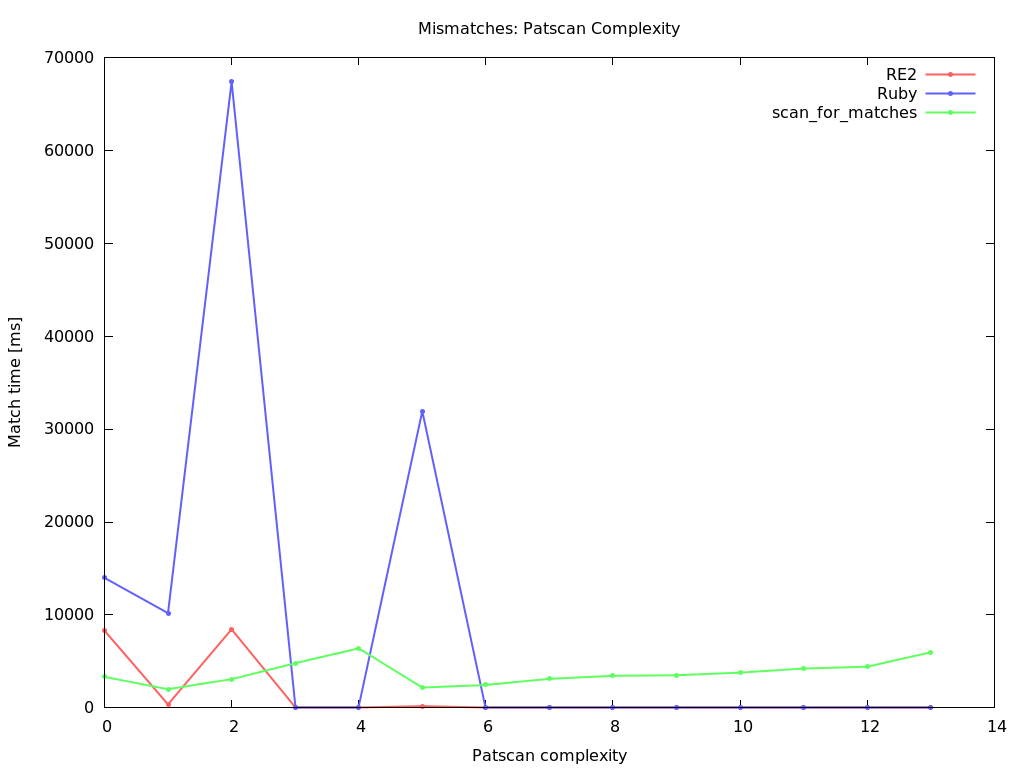
\includegraphics[scale=0.55]{graphs/mismatches.png}	
	\end{center}
	\caption{Stalin}
\end{figure}

\subsubsection{Deletions}

\subsubsection{Insertions}

\subsubsection{Combinations}

\subsubsection{Ranges}

\subsubsection{Sequences}


\newpage

\section{Conclusion (TO BE WRITTEN)}

\newpage

\pagenumbering{gobble}
\bibliographystyle{plain}
\nocite{*}
\bibliography{litterature}

\end{document}
